%1 what are the questions to answer
%2 setup (machine/code implementation/data) could be one setup per experiment or as a whole if they are identical
%3. how to perform the experiments
%4. what are the observed results
%5. what are the conclusions(discussions) from the results.

For each of the two algorithms described, we want to measure the fraction of candidate date columns that the algorithm is able to recognize. We describe a large training and experimental corpus that we collected, followed by the results of applying each algorithm to that data.
 
\subsection{Data Preparation}

The training data and test data are taken from data sets published to a free, online data analysis website. This website contains data sets that users analyzed and were interested in sharing with other people through the web. It may not be representative of data in other settings such as corporate data warehouses, but each data set is one that a user was willing to invest some time in analyzing. The published data includes both the raw data and how it was used for analysis. The service limits data sets to a maximum of 100K rows stored in a columnar database with collated strings.

We collected the contents of columns with names containing any of the following strings: Date, month, created, dt (abbreviation for date), mes (month in Spanish), datum (date in German), fecha (date in Spanish), data (date in Portuguese), and the day character used in Chinese and Japanese. Roughly 95\% of the data on the website is in English, but we attempted to include non-English data that was available. Fields of any data type other than date or datetime were analyzed, including strings, integers, and floats. One file containing the unique non-null values was created for each scanned column, and the column collation was stored in a second table.

Most database and spreadsheet systems already detect a limited set of date formats. For instance, typing the string \texttt{"12/31/1999"} into Microsoft Excel, is automatically interpreted as the date \texttt{1999-12-31}. The Microsoft Jet library \cite{Jet} used to read these text files detects a few date formats as well. Any column already converted by Excel or Jet was not included in this study.

The data was divided into two sets, one for training and one for validation. There were 30,968 files in the training set and 31,546 files in the resulting verification set.

% Should we quantify the number of formats excluded here?

\subsubsection{NULL Filtering}
Each column was then reduced to a maximum sample set of 32. We excluded domain values that appeared to be representations of \texttt{NULL}:
\begin{itemize}
\item Values containing the substring \texttt{NULL}
\item Values containing no digits and at most one non-whitespace character (\eg \texttt{" / / "})
\item Values on a list of empirically determined common \texttt{NULL} values (\eg \texttt{0000-00-00}, \texttt{NaN})
\end{itemize}
Columns that had no remaining valid samples were discarded. 

\subsubsection{Sampling}
The remaining samples were hashed and sorted on the hash value, with the top $32$ values being retained as the column's sample. We can increase the sample size if needed, but for dates, it appears to be an adequate number. In any case, the median number of non-null rows per domain in our test data is $50$, so increasing the sample size would have little benefit.

\subsubsection{Numeric Timestamps}
After NULL filtering, a common class of date representation (numeric timestamps) remained that was unsuited for parsing via our date format syntax. This included Unix epoch timestamps (expressed as second, millisecond or microsecond counts from \texttt{1970-01-01}) and Microsoft Excel timestamps (expressed fractional days since \texttt{1900-01-01}). A simple test to check that the column was numeric and inside a specific range of values representing recent dates allowed us to tag these columns to avoid analyzing them further (and incidentally to identify them for generating a simple date extraction calculation for the user.)


\subsubsection{Partial Dates}
Many of the date formats that we encountered were incomplete dates, which necessitated creating rules for what date scalar they represented.

ICU's date parsing APIs allow the specification of default values for parts when a format does not contain them. In our implementation, all time fields are set to \texttt{0} (midnight) and the date fields are set based on whether the format contains any date part specifications. When date parts are present, we use \texttt{2000-01-01} as the set of default date parts as it is the start of a leap year. When dealing with pure time formats, we model the output as a date/time and use \texttt{1899-12-30} for the date parts.

ICU will also parse Time Zones (which the algorithms recognize but the visualization system does not model) and Quarters (which we interpret as the first month of the period.) RDBMSes such as Oracle and Postgres that support time zones will be able to take advantage of  identified time zone fields.

\subsection{Evaluation}
Once the training data was analyzed, it was grouped by date format. A sample of each produced date format was manually labeled. This allowed us to quickly skip over very common formats like \texttt{MM/dd/yyyy} and focus our efforts on much less common formats. The samples were judged as to whether the produced format was reasonable and were tagged with correct formats if the produced format was unreasonable.

Further manual tagging focused on the files most likely to represent dates. Many of the files in the collection are not actually dates, such as fields named ``updated by'' (which contain ``date''). A random sample of 850 columns named exactly ``date'', ``time'' or ``month'' (case-insensitive) were manually judged.\\

\subsubsection{Minimum Descriptive Length}
Testing of the MDL algorithm was performed on a 24-core Dell T7610 running Windows 7 with the data stored on a 250GB SSD.

\begin{table}[ht]
\centering
\bgroup
\def\arraystretch{1.5}
\begin{tabular}{|p{0.48\linewidth}| p{0.24\linewidth}|}
\hline
\textbf{Number of Records} & 31,546\\ \hline
\textbf{Error Rate} & 27.95\% \\ \hline
\textbf{Analysis Speed ($\mu s$)} & 2,245.04 \\ \hline
\textbf{Validation Speed ($\mu s$)} & 1.65 \\ \hline
\textbf{Median Not Null} & 50 \\ \hline
\end{tabular}
\egroup
\label{tab:mdlstats}
\caption{MDL Parsing Statistics.}
\end{table}

To test the MDL algorithm, we ran it over the set of samples from each validation file to generate a ranked list of formats for the file. Each format was then applied to the entire file's data set, recording both the number of errors and the elapsed times. In cases where we generated multiple formats and the main format produced errors, we applied the second format to the unparsed strings. The summary statistics from this processing are presented in Table 2.

The analysis speed is the average time needed per sample for structure extraction. At 2.5ms, this is well below most human perceptual thresholds for a set of 32 samples, so any latency in command execution would be restricted to the ability of the underlying database to provide the samples for analysis in a timely manner. (As a column store, the database can often supply such domains without a full table scan, further improving responsiveness.) 

The validation speed is the average time needed to parse a value, and provides an estimate of how fast the ICU implementation can process string values into scalars and works out to 620K values per core per second.\\
 
\begin{figure}[ht]
\centering
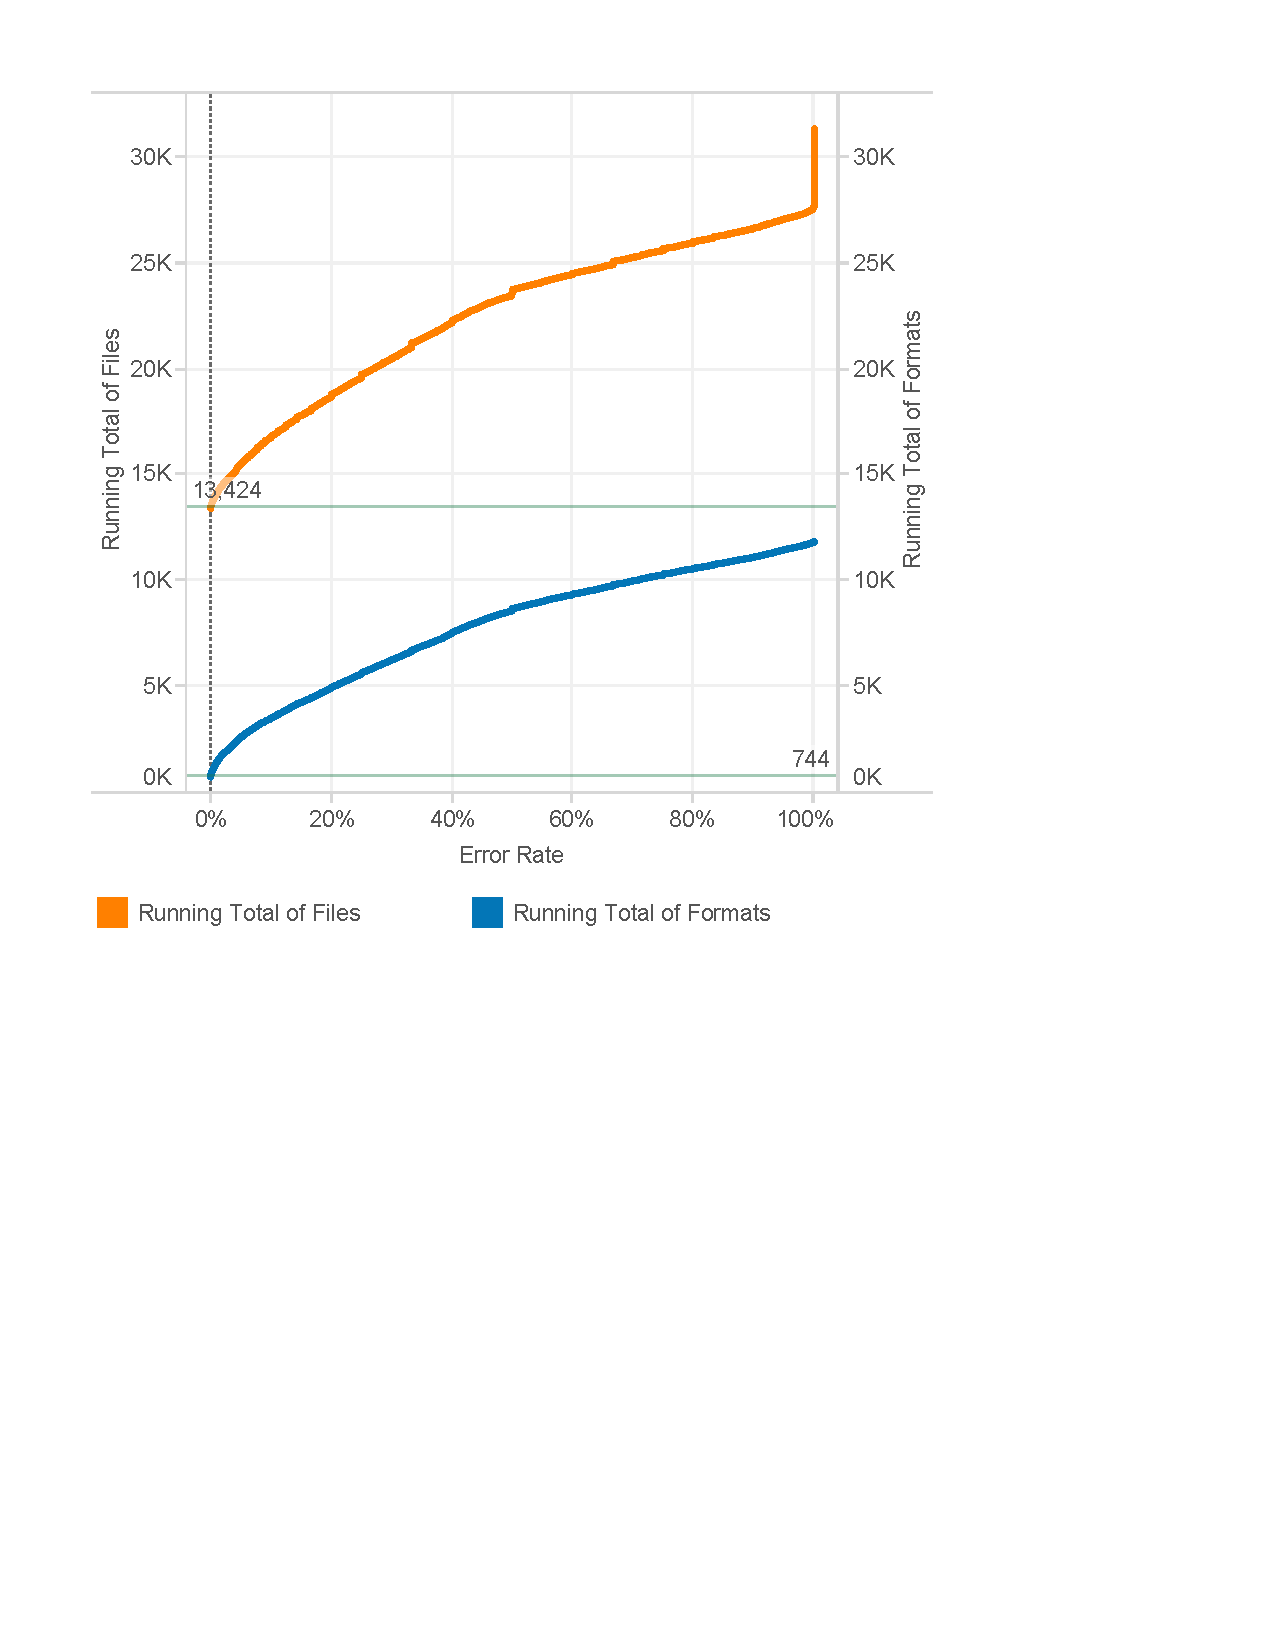
\includegraphics[width=\columnwidth]{figures/FigureM2}
\caption{MDL Error Rate}
\label{fig:M2}
\end{figure}


The error rate reflects the fact that only about 40\% of the files have an associated format that parses the non-null values without error. To examine the error rate in greater detail, we turn now to Figure \ref{fig:M2}.

On the left hand side, we can see that the algorithm found 744 distinct formats that parsed 13,424 files with no error. This is a remarkable number of valid formats and underscores the need for this kind of algorithm. Raising the error rate threshold to 5\% results in about 2500 formats found in 15,000 files, or nearly half of the files. 

What do these formats look like? Figure \ref{fig:M3} shows a histogram of the 25 most common formats containing a year format code at the 5\% threshold, color-coded by error rate. (A sample value is provided to the right of each bar for illustrative purposes.) The formats have also been filtered to files with at least 5 samples. Most of the samples are clearly dates with a wide range of formats (the format where the time zone is between the time and the year is surprisingly common.)
 
\begin{figure}[ht]
\centering
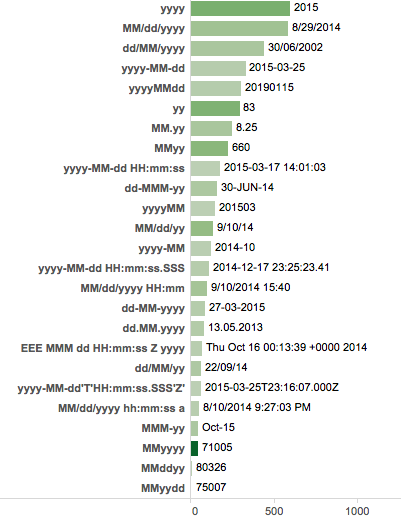
\includegraphics[width=\columnwidth]{figures/FigureM3}
\caption{MDL Output}
\label{fig:M3}
\end{figure}


Some of the dates are clearly just numbers, but our approach is to assume that when the user tells us that the column contains dates we should find the best fit. The samples include dates from a wide range of historical sources (\eg Roman pottery dates) so we have elected to defer the date identification task to the user.

\subsubsection{Natural Language Processing}


We implemented the grammar, training and parsing in Python 3.4.1 using the Natural Language Toolkit libraries~\cite{nltk} on a quad core Dell T7600 running Windows 7. The complexity of the CYK parsing algorithm is $O(n^{3}|G|)$, where $n$ is the length of the input and $|G|$ is the size of the grammar~\cite{Younger67}. The PCFG grammar uses a set of $22$ phrase-level non-terminals and $30$ terminals to classify the various constituents in the corpus. Because the CYK algorithm finds the maximum likelihood solution, there are no search errors (rather probability $p = 0$, and a modification in the grammar is required to improve accuracy.

Similar to the MDL algorithm described in the previous subsection, the CYK parser is run over the same set of samples from each validation file to generate a ranked list of parse trees representing the date-time formats. As a second pass of the parser, starting from the most probable parse tree, each parse tree is then applied to the entire file's columnar data to determine the dominant pattern(s). For the second pass, we can parallelize the CYK parsing because the dependencies between reapplying the ranked list of parse trees are very sparse.

The initial average parsing speed to compute the ranked set of probable parse trees is $0.93s$, while the average time taken to compute the overall dominant pattern(s) for the entire column of data is $1.4s$. While the natural language parsing implementation is in Python as the NLTK package is easily configurable, we could expect greater speed-up in parsing performance by employing C/C++ CYK parsing libraries.


Out of the $31,546$ files used for testing, the NLP parser identified a dominant format for $26, 534 (84.11\%)$ where $p >= 0.5$. $1634$ unique formats were identified. Figure \ref{fig:NLP1} shows a histogram of the most common formats identified containing \texttt{Year}. There are some variations compared to Figure \ref{fig:M3} including the fact that we are not filtering the results by any error rate in the NLP parsed results.

\begin{figure}[ht]
\centering
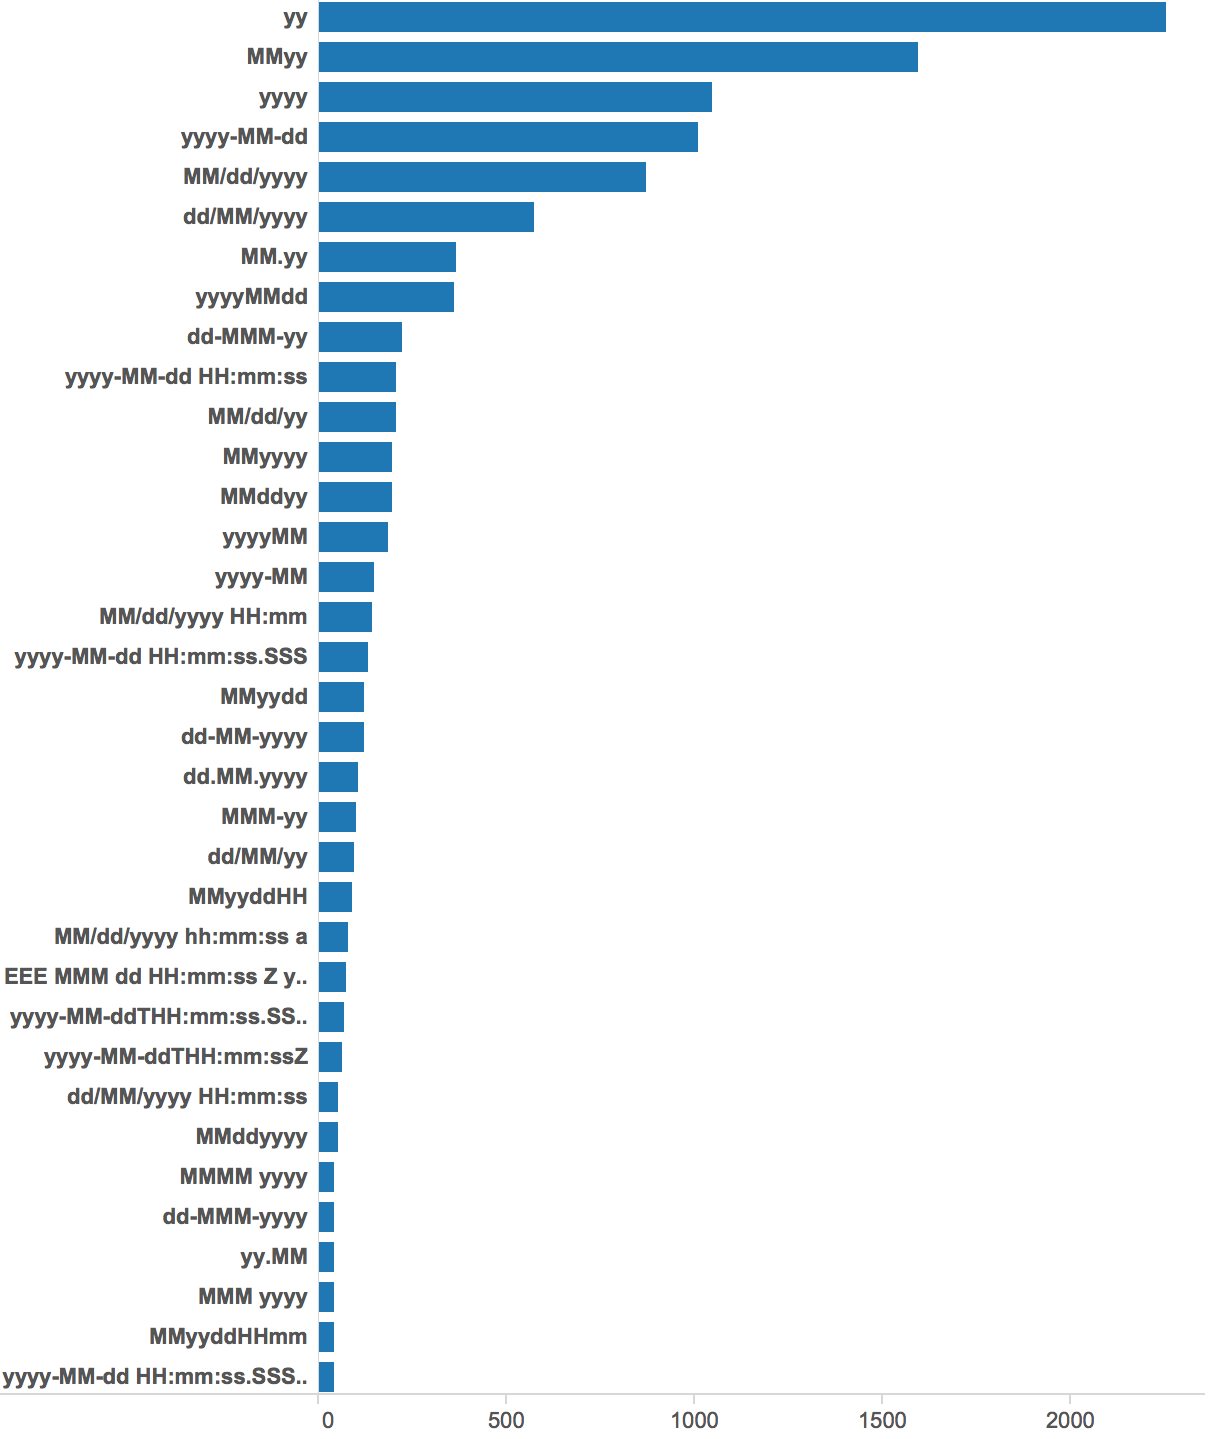
\includegraphics[width=\columnwidth]{figures/FigureNLP1}
\caption{Most common date formats identified by the NLP algorithm.}
\label{fig:NLP1}
\end{figure}

\subsubsection{Cross-Checking}
We compared the results of the minimum description length and natural language processing algorithms. The two algorithms match for 97.9\% of our validation set. The main differences in the results are due to small differences in the implementations. The minimum description length implementation recognizes formats with leading plus and minus signs, but these are almost certainly numbers, not dates. The minimum description length implementation also recognizes the Excel date formats, but this was not supported by the natural language implementation. There was one file that contained formats such as \texttt{`Fall 2000'} and \texttt{`Spring 2000'}, and the two algorithms picked different seasons in their format. One other file contained a set of integers that are not actually dates, and one algorithm picked \texttt{MMyyyy} format, while the other picked \texttt{HHmmss} format.

\subsubsection{Production}

Although both algorithms achieved comparable high accuracies in parsing date time strings, we utilized the minimum description length method in the production code of our system. This was primarily due to the fact that the MDL algorithm was written in C++, allowing for higher performance. We believe that NLP version if written in C++ as opposed to Python, would lead to better performance. 